\section{Appendix/Discarded}
\begin{figure*}[ht!]
    \centering
    \begin{subfigure}[t]{0.32\textwidth}
        \centering
        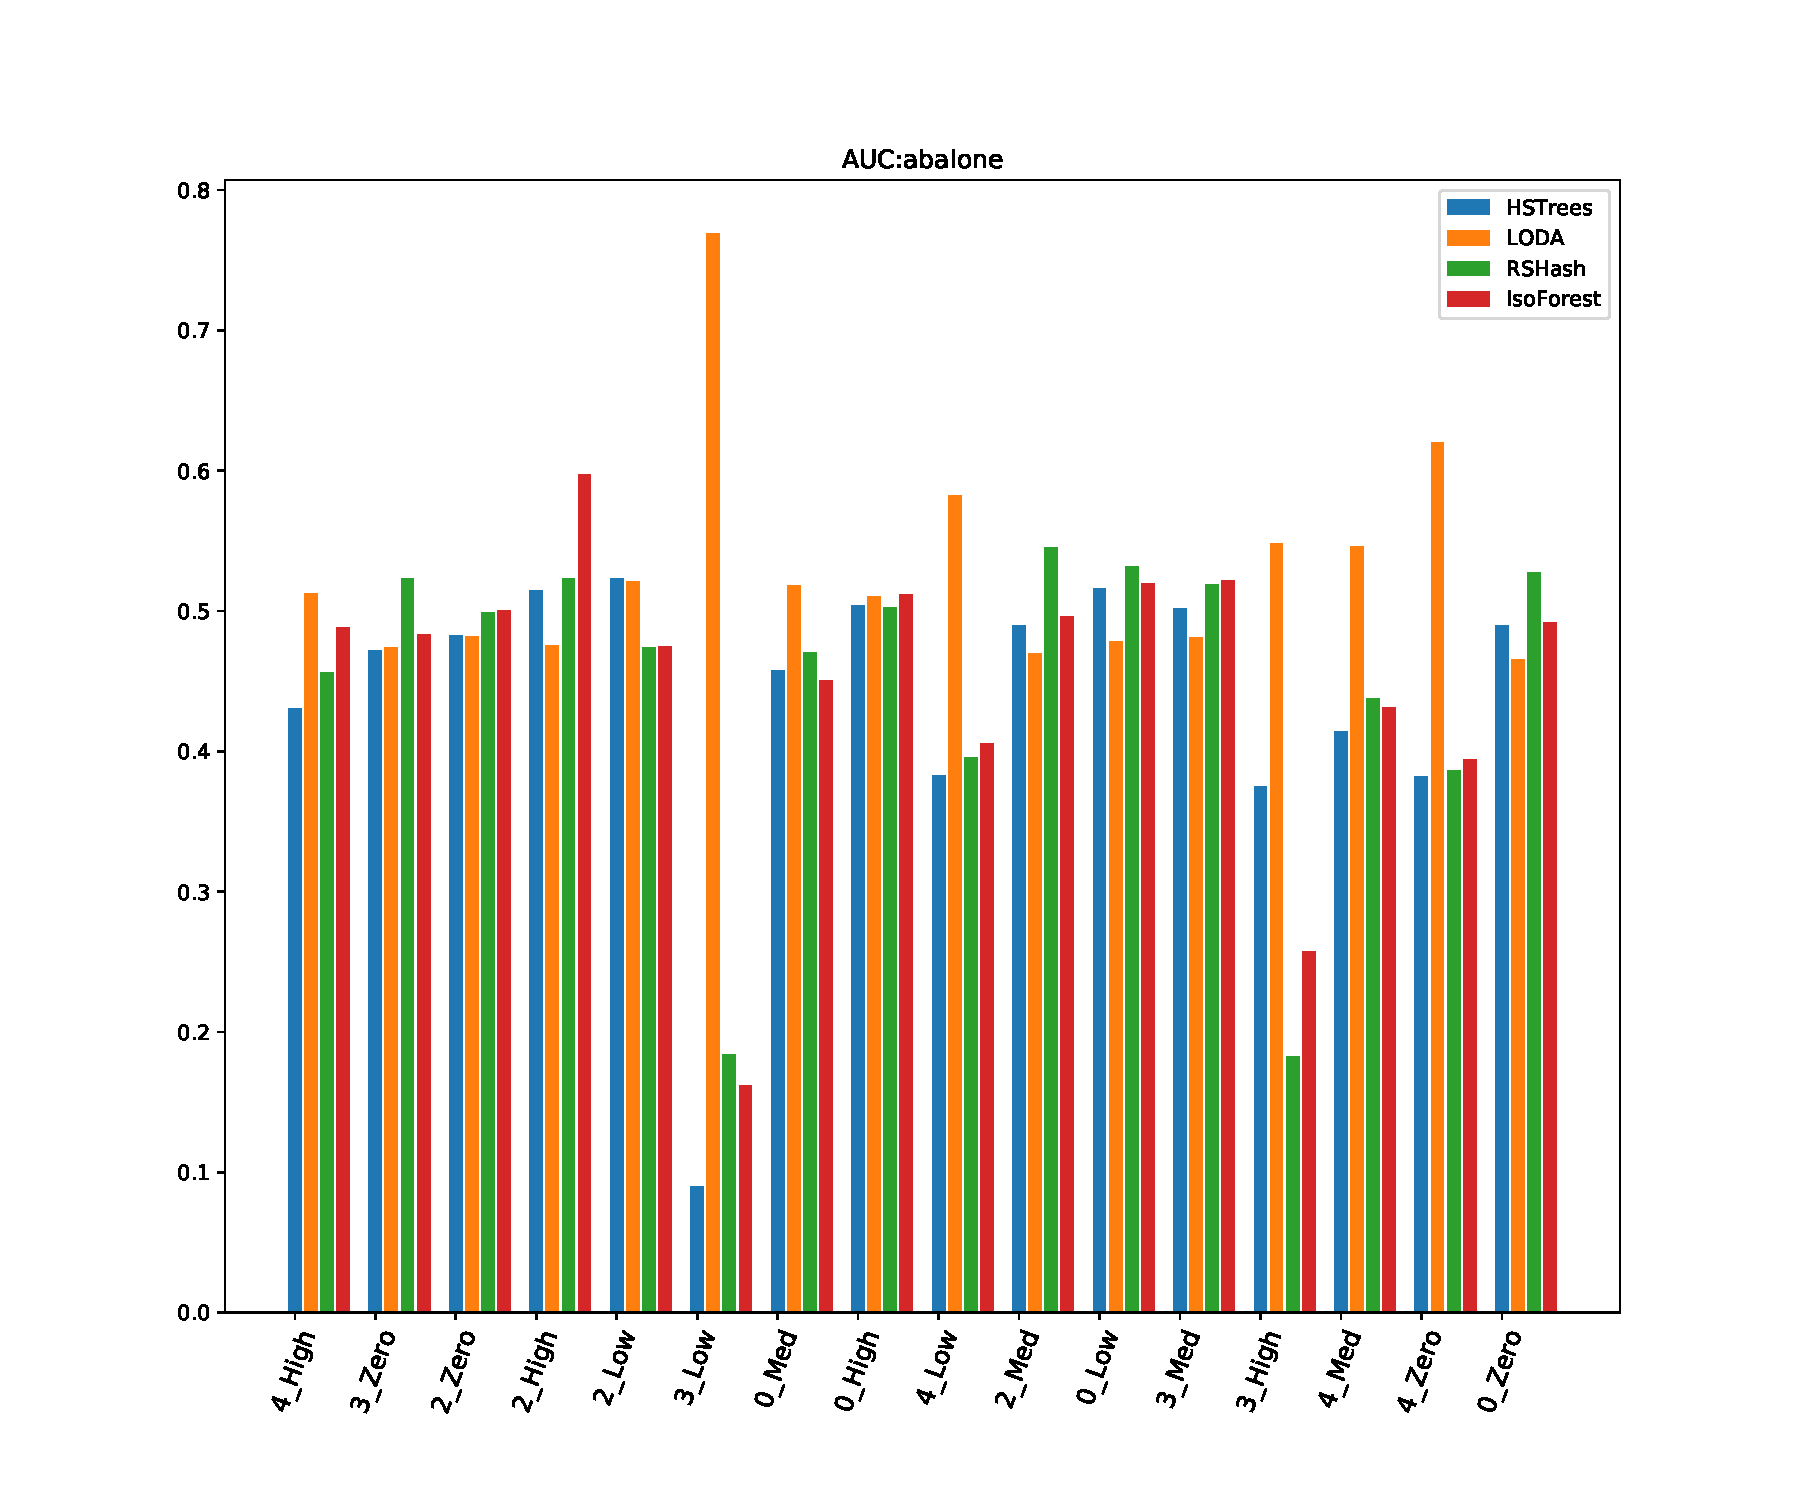
\includegraphics[width=\linewidth]{fig/baseline/abalone.pdf}
        \caption{AUC - ABALONE}
    \end{subfigure}
    \hfill
    \begin{subfigure}[t]{0.32\textwidth}
        \centering
        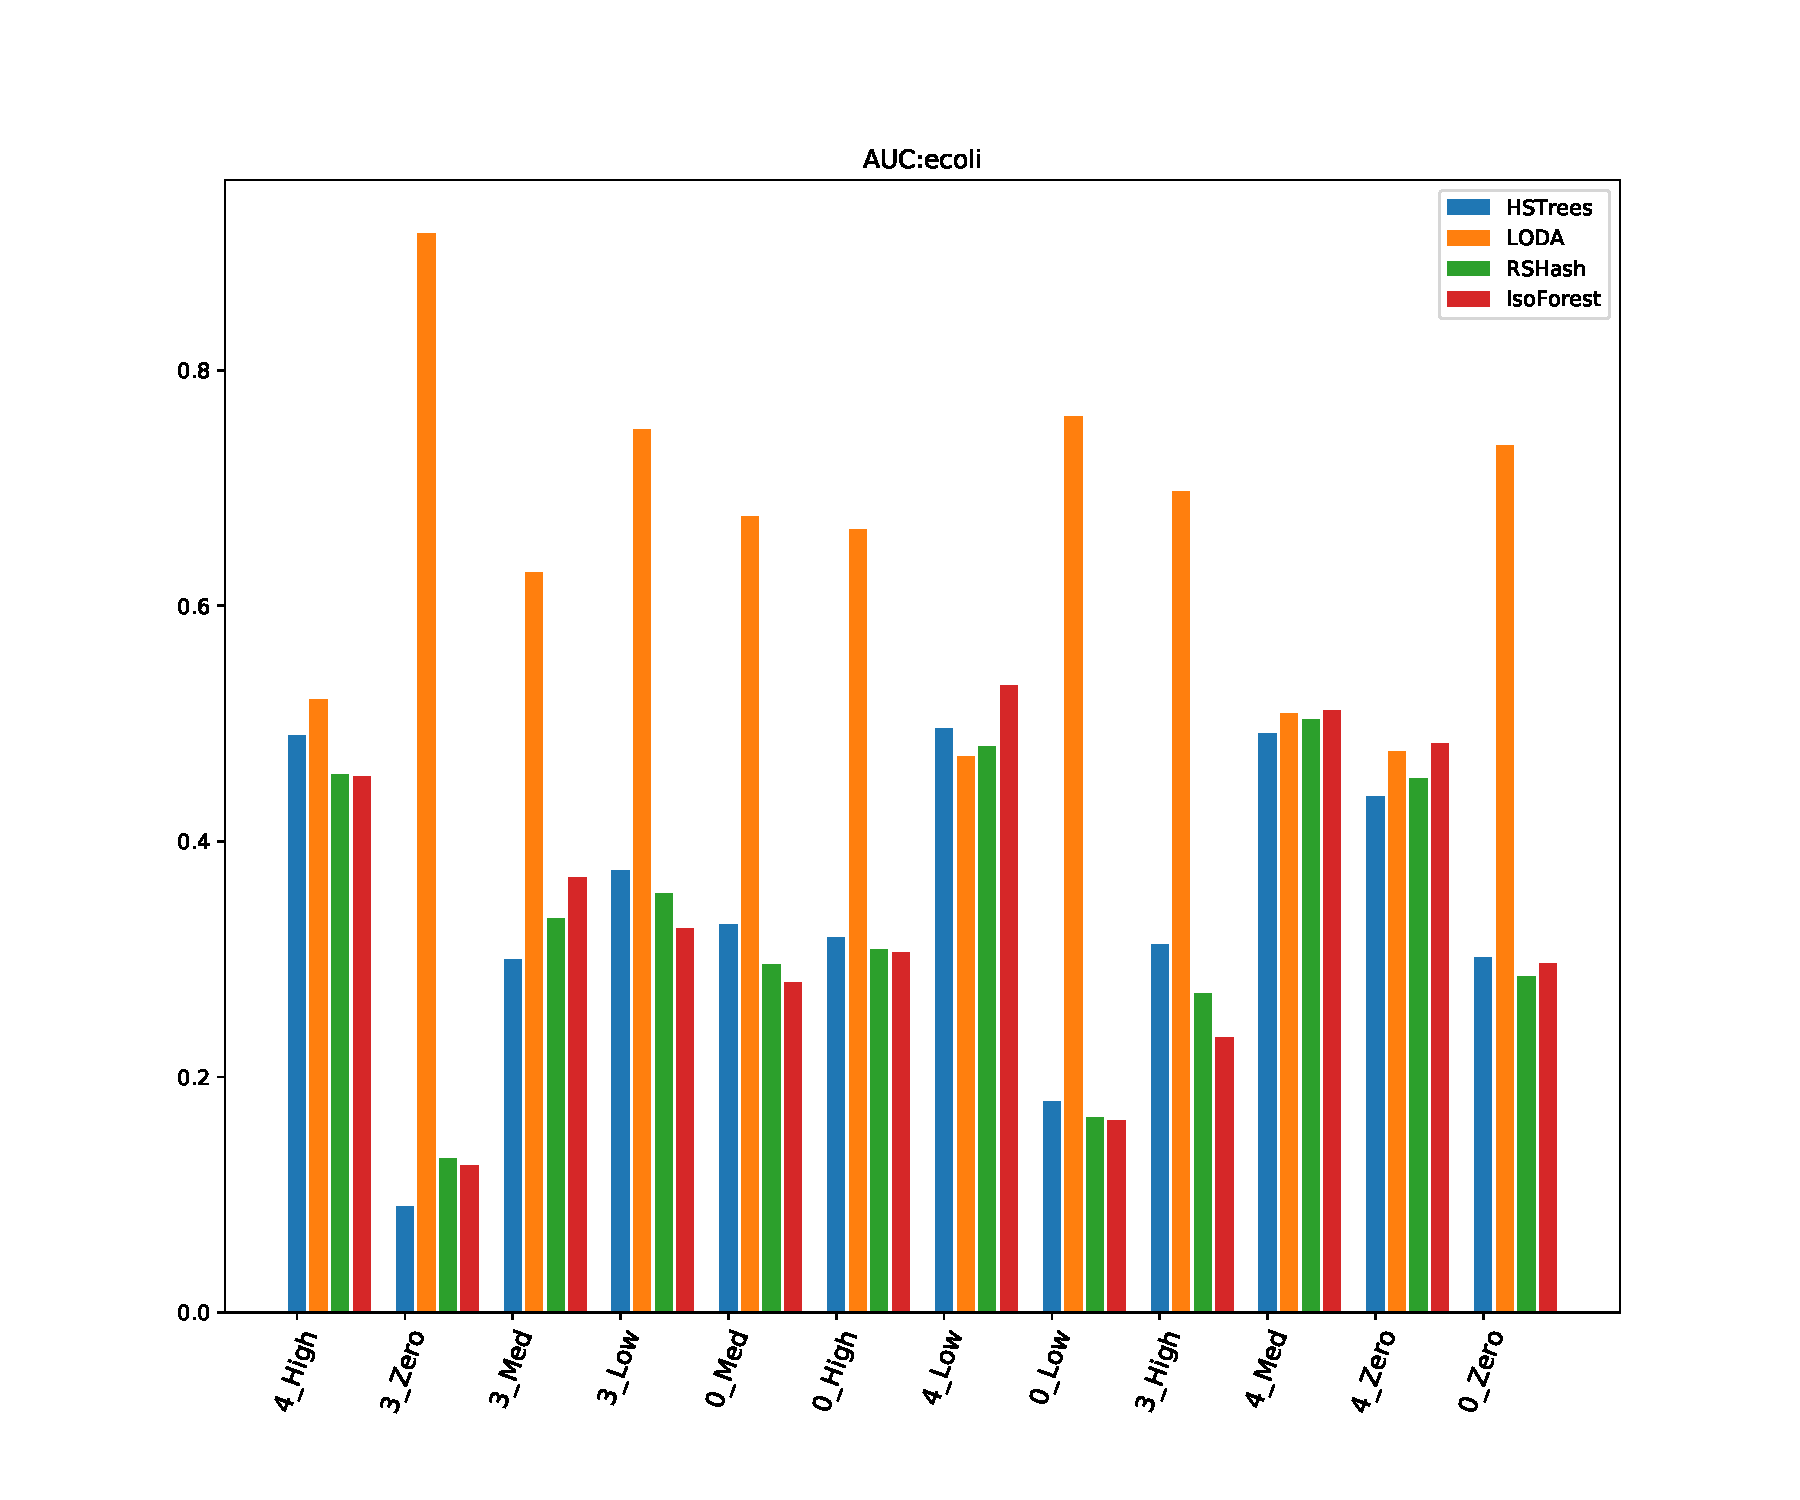
\includegraphics[width=\linewidth]{fig/baseline/ecoli.pdf}
        \caption{AUC - ECOLI}
    \end{subfigure}
		\hfill
    \begin{subfigure}[t]{0.32\textwidth}
        \centering
        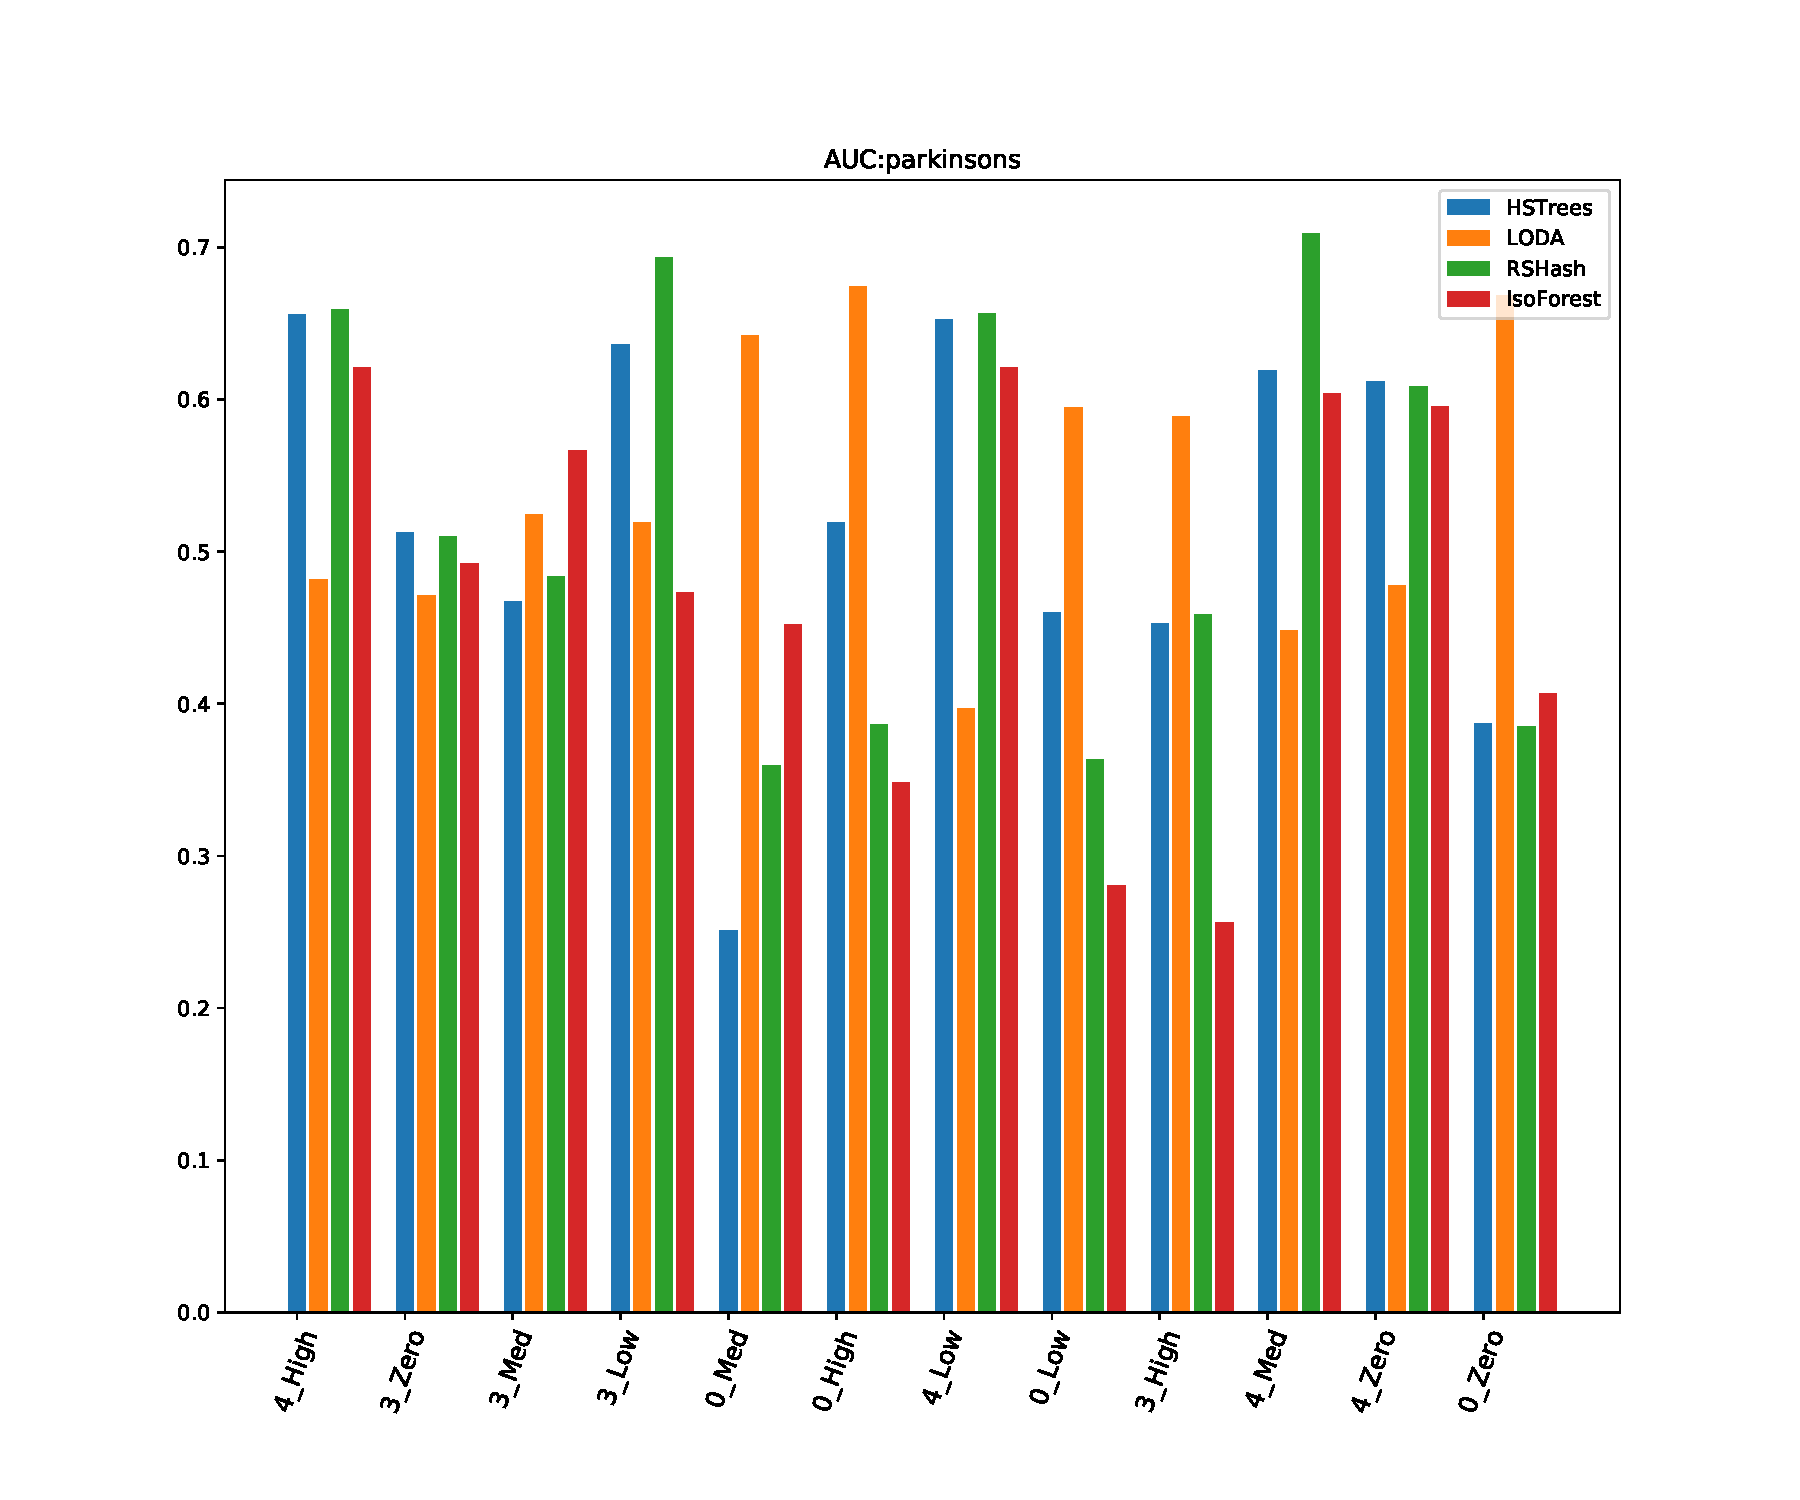
\includegraphics[width=\linewidth]{fig/baseline/parkinsons.pdf}
        \caption{AUC - Parkinsons}
    \end{subfigure}
		\hfill
    \caption{Baseline Performance on Feature Irregular Benchmark datasets}
\end{figure*}

\begin{figure*}[ht!]
    \centering
    \begin{subfigure}[t]{0.32\textwidth}
        \centering
        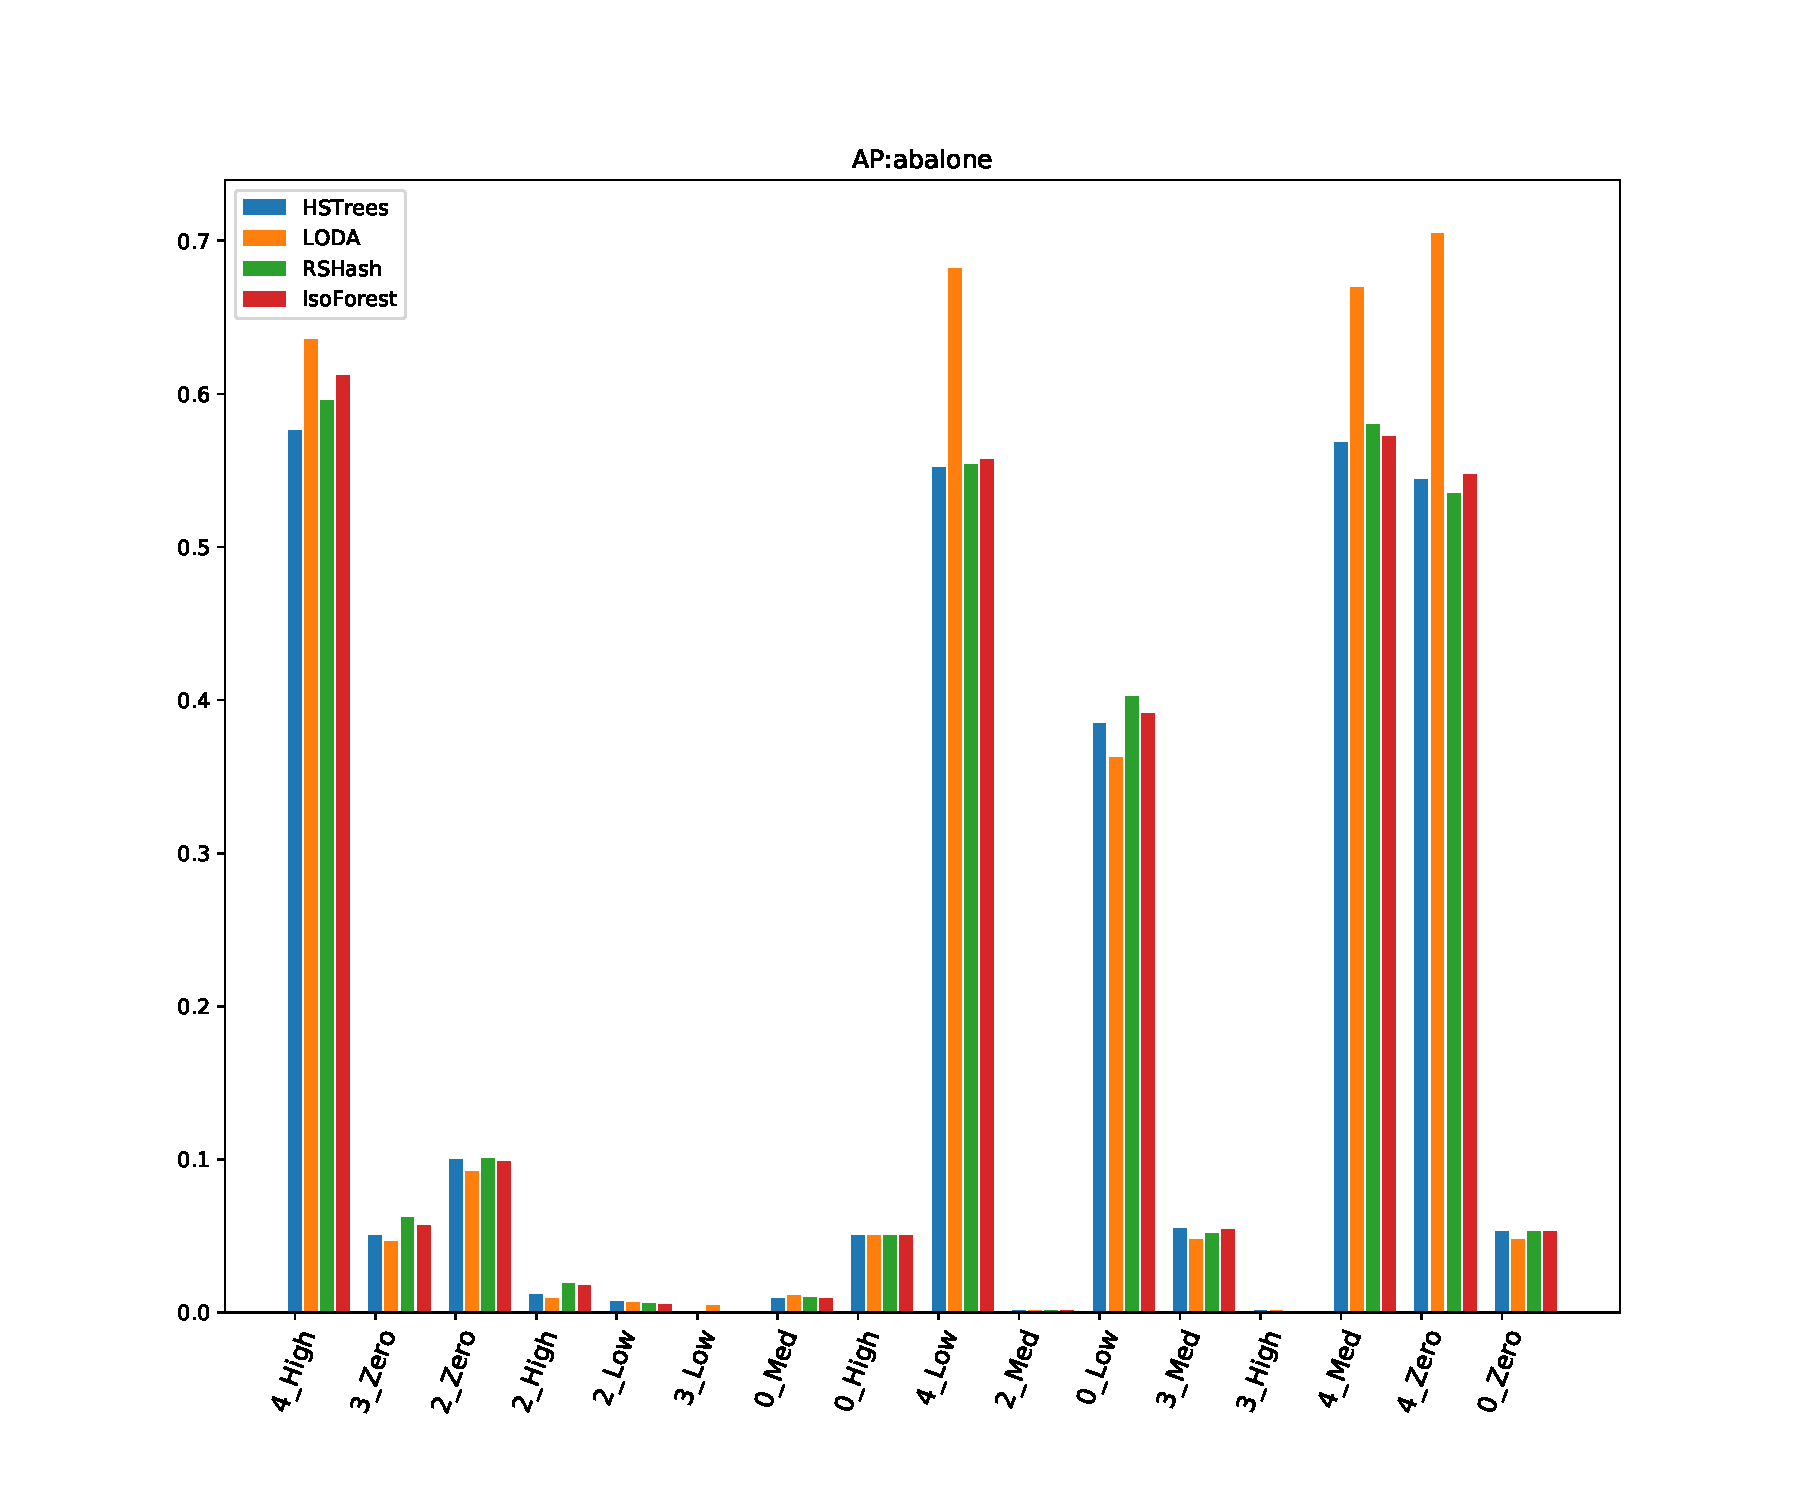
\includegraphics[width=\linewidth]{fig/baseline/AP_abalone.pdf}
        \caption{AP - ABALONE}
    \end{subfigure}
    \hfill
    \begin{subfigure}[t]{0.32\textwidth}
        \centering
        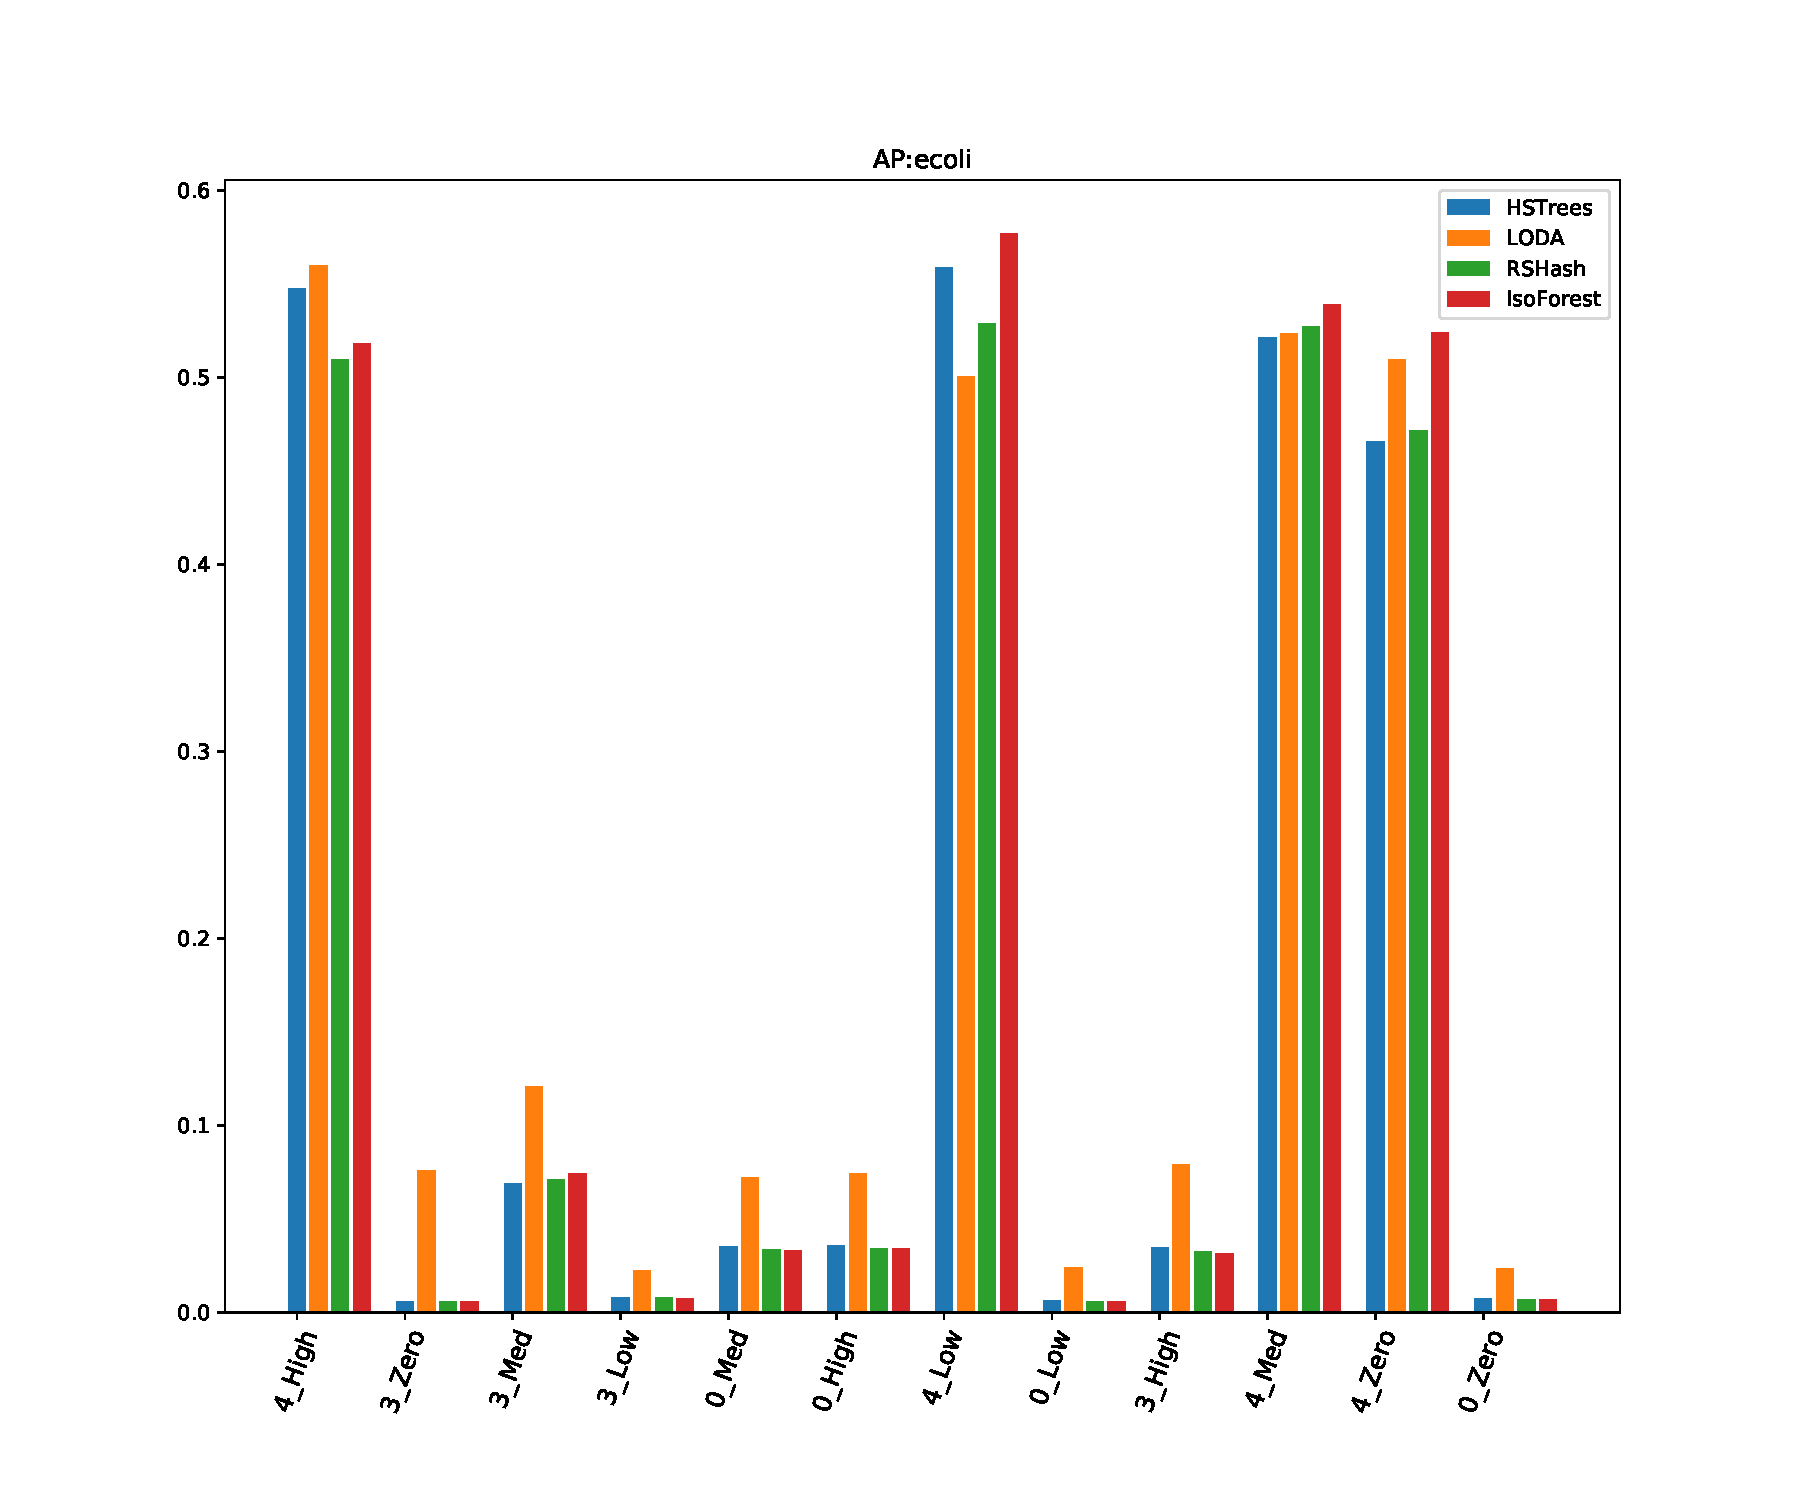
\includegraphics[width=\linewidth]{fig/baseline/AP_ecoli.pdf}
        \caption{AP - ECOLI}
    \end{subfigure}
		\hfill
    \begin{subfigure}[t]{0.32\textwidth}
        \centering
        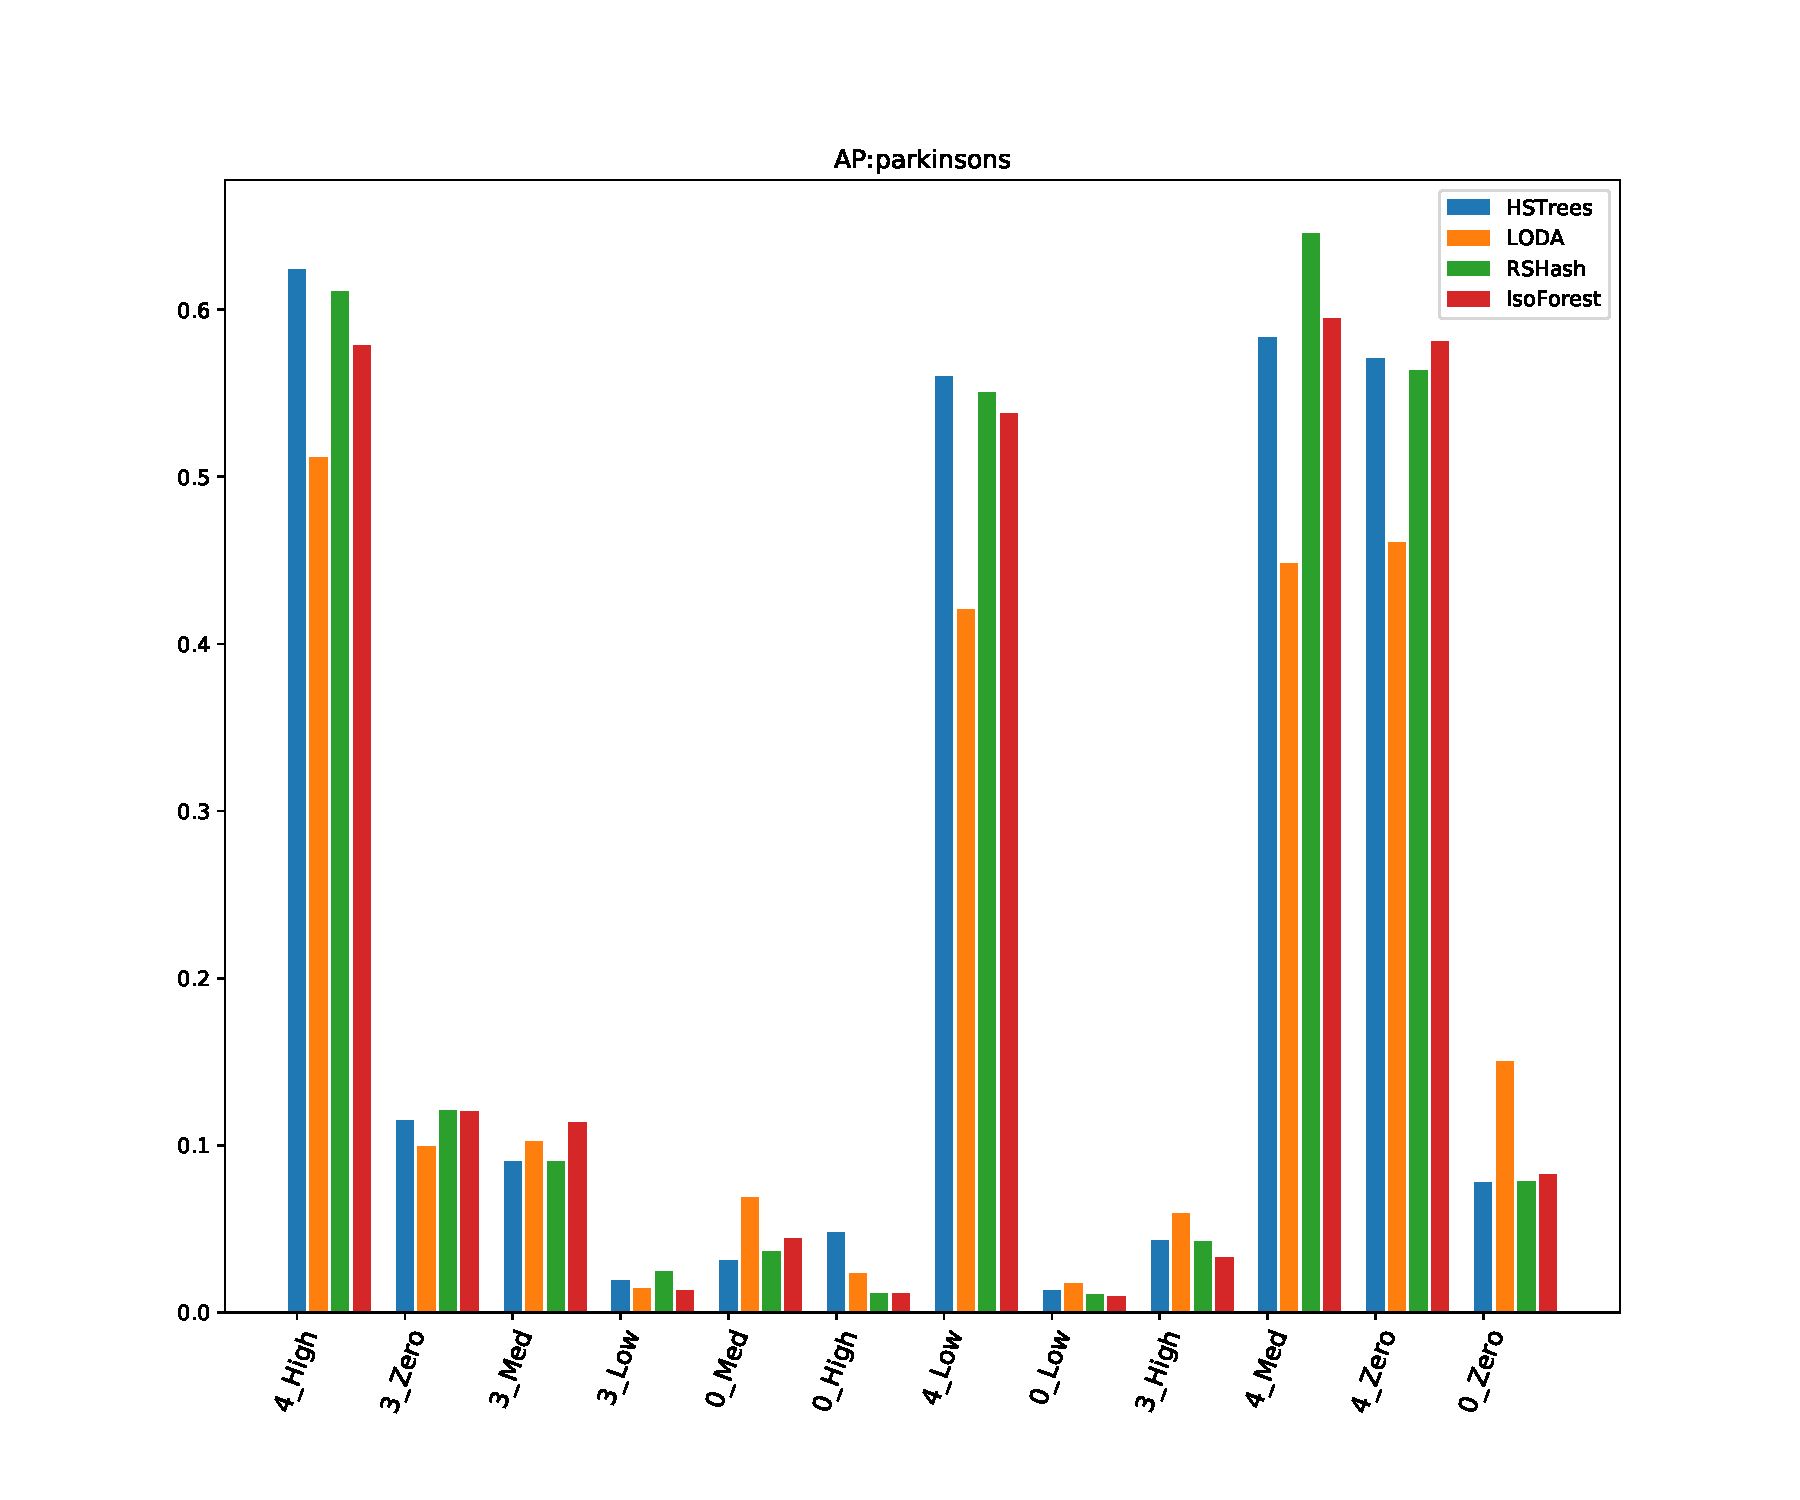
\includegraphics[width=\linewidth]{fig/baseline/AP_parkinsons.pdf}
        \caption{AP - Parkinsons}
    \end{subfigure}
		\hfill
    \caption{Baseline Performance on Feature Irregular Benchmark datasets}
\end{figure*}

\begin{table}
\centering
\caption{Some benchmark datasets. Square brackets indicate number of datasets of each type.}
\label{table:benchmark}
\begin{tabular}{|c|c|c|c|}
\hline
\textbf{Dataset Name} & \textbf{Point Difficulty Range}                         & \textbf{Feature Irrelevance}                          & \textbf{\#Datasets} \\	\hline
abalone               & PD-0 {[}4{]}, PD-2 {[}4{]} , PD-3 {[}4{]}, PD-4 {[}4{]} & Regular{[}4{]}, 1.2{[}4{]}, 1.5 {[}4{]}, 2.0{[}4{]}   & 16                  \\	\hline
ecoli                 & PD-0 {[}4{]}, PD-3 {[}4{]}, PD-4 {[}4{]}                & Regular{[}3{]}, 1.2 {[}3{]}, 1.5 {[}3{]}, 2.0 {[}3{]} & 12                  \\	\hline
parkinsons            & PD-0 {[}4{]}, PD-3 {[}4{]}, PD-4 {[}4{]}                & Regular{[}3{]}, 1.2 {[}3{]}, 1.5 {[}3{]}, 2.0 {[}3{]} & 12                 \\	\hline
\end{tabular}
\end{table}

For low and mid-dimensional dataset, pick only datasets perform good (AUC $>$ 0.7)
\begin{itemize}
\item{Low-dimensional dataset (n=1)}: Add noisy columns. Gaussian noise with $0.01$average mean, $0.01$average variance of existing features. Level of noise = 100\%, 1000\% of features, or noise strength = $0.01$,$0.1$.
\item{Medium - dimensional dataset (n=2)}: Add noisy columns. Gaussian noise with average mean, average variance of existing features. Level of noise = 100\%, 1000\% of features.
\item{High-dimensional dataset (n=3)}: Take only normal points. Choose $k=1$\% of rows, and $m$\% of features, add gaussian noise to just this sub-block. Level of noise is controlled by $k$, $m$ and strength of Gaussian noise (mean, variance).
\end{itemize}

\begin{table}[ht!]
    \centering
		\begin{tabular}{llllll}
				\toprule
				\textbf{Dataset} & \textbf{iForest AP} &  \textbf{LODA-AP} & \textbf{RSH-AP} &  \textbf{HST-AP} \\
				\midrule
				\multicolumn{3}{c}{\textit{High-dimensional Datasets}}\\
				Madelone & $0.516 $ & $0.524$ & $0.507$ & $0.500$\\
				Madelone-Noisy (5.0, 0.1, 10.0) & $0.837$ & $0.985$ & $0.918$ & $0.691$	\\
				Madelone-Noisy (5.0, 0.1, 20.0) & $0.299$ & $0.179$ & $0.312$ & $0.292$	 \\
				Madelone-Noisy (5.0, 0.1, 50.0) & $0.112$ & $0.116$ & $0.114$ & $0.102$	\\
				\midrule
				Letter-Recognition & $0.4713$ & $0.461$ & $0.460$ & $0.4513$	\\
				Letter-Recognition-Noisy (5.0, 0.1, 10.0) & $0.108$ & $0.104$ & $0.1067$ & $0.102$	\\
				Letter-Recognition-Noisy (5.0, 0.1, 20.0) & $0.114$ & $0.105$ & $0.1090$ & $0.104$	\\
				Letter-Recognition-Noisy (5.0, 0.1, 50.0) & $0.113$ & $0.110$ & $0.110$ & $0.108$	\\
				\midrule
				Gisette & $0.4217$ & $0.4442$ & $0.4239$ & $0.438$	\\
				Gisette-Noisy (5.0, 0.1, 10.0) & $0.1036$ & $0.098$  & $0.1342$ & $0.097$	\\
				Gisette-Noisy (5.0, 0.1, 20.0) & $0.1176$ & $0.105$ & $0.1220$ & $0.1141$	\\
				Gisette-Noisy (5.0, 0.1, 50.0) & $0.1041$ & $0.096$ & $0.109$ & $0.095$	\\
				\midrule
				Isolette & $0.4693$ & $0.434$ & $0.433$ & $0.415$	\\
				Isolette-Noisy (5.0, 0.1, 10.0) & $0.116$ & $0.1175$ & $0.1317$ & $0.117$	\\
				Isolette-Noisy (5.0, 0.1, 20.0) & $0.0956$ & $0.0934$ & $0.093$ & $0.0937$	\\
				Isolette-Noisy (5.0, 0.1, 50.0) & $0.094$ & $0.0992$ & $0.096$ & $0.097$	\\
				\bottomrule
		\end{tabular}
		\caption{AP for Baselines.}
\end{table}

\begin{table}[ht!]
    \centering
		\begin{tabular}{lllll}
				\toprule
				\textbf{Dataset} & \textbf{iForest-AP} & \textbf{LODA-AP} & \textbf{RSHash-AP} & \textbf{HSTree-AP}	\\
				\midrule
				\multicolumn{3}{c}{\textit{Low/medium-dimensional Datasets}}\\
				Breast-Cancer-Wisconsin & $0.662 \pm 0.024$ & $ 0.881 \pm 0.011$ & $0.727 \pm 0.018$ & $0.729 \pm 0.007$\\
				Breast-Cancer-Wisconsin-Noisy (100, 0.1) & $0.656 \pm 0.03$ & $ 0.84 \pm 0.016$ & $ 0.7018 \pm 0.015$ & $ 0.756 \pm 0.018$	\\
				Breast-Cancer-Wisconsin-Noisy (1000, 0.1) & $0.4798 \pm 0.04$ & $ 0.734\pm 0.04$ & $0.539 \pm 0.04$ & $ 0.463 \pm 0.021$	\\
				Breast-Cancer-Wisconsin-Noisy (2000, 0.1) & $0.457 \pm 0.049$ & $ 0.668\pm 0.039$ & $0.46 \pm 0.04$ & $ 0.488 \pm 0.017$	\\
				Breast-Cancer-Wisconsin-Noisy (5000, 0.1) & $0.395 \pm 0.0167$ &  $0.518 \pm 0.064$ & $0.4059 \pm 0.03$ & $ 0.378 \pm 0.015$	\\
				\midrule
				Ionosphere & $0.810 \pm 0.007$ & $ 0.788 \pm 0.023$ & $ 0.788 \pm 0.023 $ & $0.798 \pm 0.001$\\
				Ionosphere (100, 0.1) & $0.595 \pm 0.042$ & $0.768 \pm 0.016$ & $0.734 \pm 0.018$ & $0.728 \pm 0.006$	\\
				Ionosphere (1000, 0.1) & $0.7535 \pm 0.011$ & $0.737 \pm 0.011$ & $0.537 \pm 0.048$ & $0.578 \pm 0.008$	\\
				Ionosphere (2000, 0.1) & $0.496 \pm 0.04$ &  $0.718 \pm 0.025$ & $0.432 \pm 0.04$ & $0.422 \pm 0.005$	\\
				Ionosphere (5000, 0.1) & $0.394 \pm 0.02$ &  $0.681 \pm 0.038$ & $0.387 \pm 0.036$ & $0.399 \pm 0.0105$	\\
				\midrule
				Magic-Telescope & $0.638 \pm 0.01$ & $0.624 \pm 0.012$ & $0.657 \pm 0.008$ & $0.632 \pm 0.005$\\
				Magic-Telescope (100, 0.1) & $0.4551 \pm 0.02$ & $0.615 \pm 0.009$ & $0.598 \pm 0.013$ & $0.574 \pm 0.004$	\\
				Magic-Telescope (1000, 0.1) & $0.5908 \pm 0.006$ & $0.604 \pm 0.005$ & $0.465 \pm 0.028$ & $0.425 \pm 0.006$	\\
				Magic-Telescope (2000, 0.1) & $0.413 \pm 0.014$  & $ 0.588 \pm 0.005$ & $0.434 \pm 0.023$ & $ 0.3735 \pm 0.004$	\\
				Magic-Telescope (5000, 0.1) & $0.372 \pm 0.004$  & $ 0.522 \pm 0.022$ & $0.384 \pm 0.019$ & $ 0.3710 \pm 0.0014$	\\
				\midrule
				Pima-Indians & $0.499 \pm 0.01$ & $0.470 \pm 0.021$ & $0.521 \pm 0.006$ & $0.4992 \pm 0.0098$\\
				Pima-Indians (100, 0.1) & $0.395 \pm 0.022$ & $0.4680 \pm 0.0177$ & $0.49 \pm 0.016$ & $0.4598 \pm 0.015$	\\
				Pima-Indians (1000, 0.1) & $0.471 \pm 0.01$ & $0.454 \pm 0.014$ & $0.397 \pm 0.014$ & $0.383 \pm 0.009$	\\
				Pima-Indians (2000, 0.1) & $0.369 \pm 0.02$ &  $0.419 \pm 0.015$ & $0.363 \pm 0.0105$ & $0.373 \pm 0.007$	\\
				Pima-Indians (5000, 0.1) & $0.351 \pm 0.017$  & $0.408 \pm 0.027$ & $0.355 \pm 0.02$ & $0.331 \pm 0.002$	\\
				\bottomrule
		\end{tabular}
		\caption{AP over 10 runs}
\end{table}
